\documentclass[11pt,a4paper]{article}
\usepackage{fontspec,amsmath,amssymb,bm,graphics,graphicx}
\usepackage{float}
\usepackage{multicol}
\newcommand{\tabincell}[2]{\begin{tabular}{@{}#1@{}}#2\end{tabular}} %usage \tabincell{c}{Total number \\of the characters}
\usepackage[margin=2cm]{geometry}
\setmainfont{cwTeX 明體}
\XeTeXlinebreaklocale "zh"
\XeTeXlinebreakskip = 0pt plus 1pt

\title{User Manual}
\author{彭陸,李韋翰,葉佳隆}
\date{}

\begin{document}
\maketitle
\section{基本功能}
\begin{itemize}
\item 內建10種燈號狀態,且同時顯示此狀態之可停留時間及剩餘時間。
\item 可自由切換至下一種燈號狀態。
\item 可自由增減任一狀態之可停留秒數。
\item 可暫停。
\item 提供小綠人顯示目前狀態可否可通行。
\end{itemize}

\section{面板說明}
\begin{figure}[H]
  \centering
  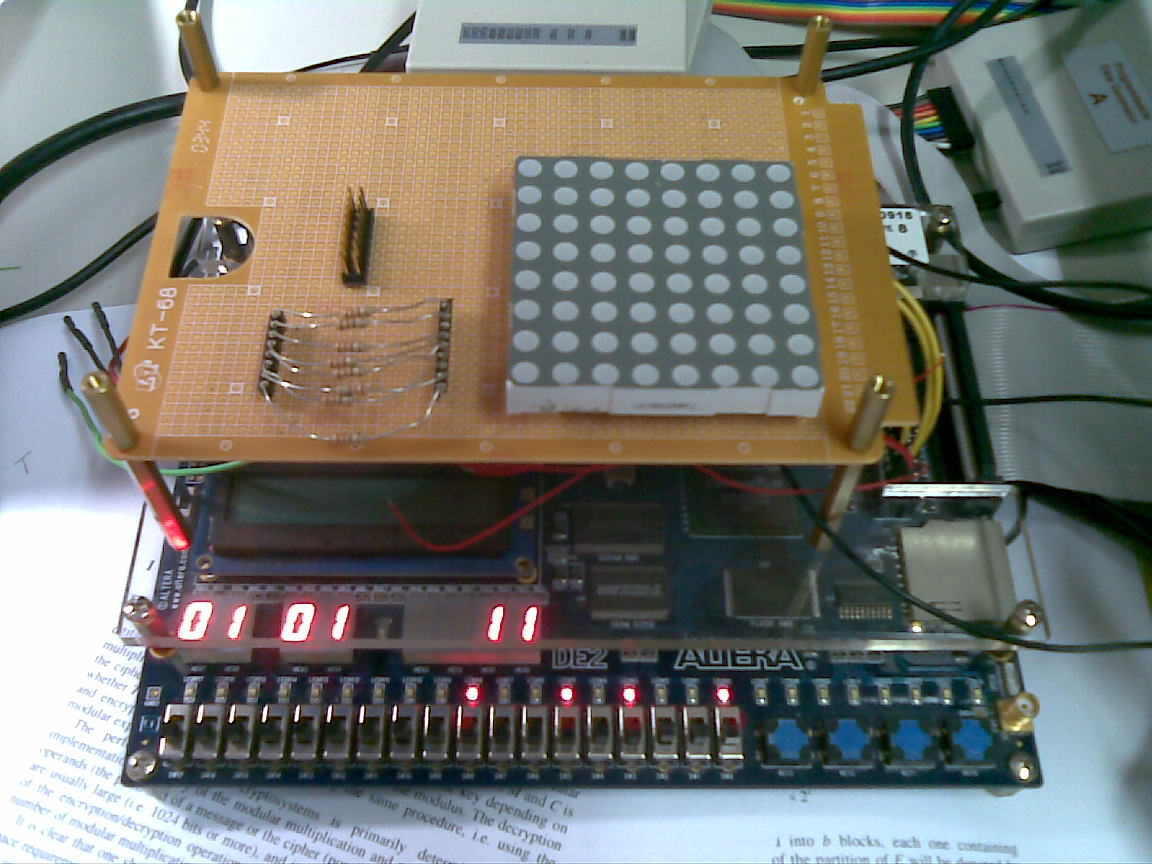
\includegraphics[width=7cm]{panel}
  \caption{Panel}
\end{figure}
\begin{multicols}{2}
\begin{itemize}
\item 右下角之4個按鈕
  \begin{itemize}
\item Key0:跳至下一燈號狀態
\item Key1:暫停
\item Key2:增加目前狀態之可停留時間1秒
\item Key3:減少目前狀態之可停留時間1秒
  \end{itemize}

\item 三組7段顯示燈號
  \begin{itemize}
    \item 左:目前狀態之剩餘秒數
    \item 中:目前狀態之可停留時間
    \item 右:目前所在的燈號狀態編號  
  \end{itemize}
\item 小綠人燈號:顯示目前可否通行
\item 最左邊兩個led燈號,切換狀態指示燈,暫停燈。
\item 最左下角的按鈕由左到右為reset,編輯模式,刪除狀態。
\item 燈號下的按鈕為編輯燈號的按鈕。
\end{itemize}  
\end{multicols}

\section{基本操作說明}

\subsection{燈號變化}
啟動號,燈號狀態便會開始變化,其相關訊息會顯示再面板中的七段顯示器上。這時可以使用右下角的四個按鈕控制他。key3可以減少目前狀態的停留秒數、key2可以增加目前狀態的停留秒數。key1是暫停,key0是到下一個狀態,若一直按住key0則會每秒前進一個狀態。

\section{進階功能}
\begin{itemize}
\item 可插入新的燈號狀態直至16個。
\item 可刪除任意的燈號狀態。
\end{itemize}

\section{進階功能操作說明}

\subsection{插入燈號狀態}
在想插入狀態的燈號處撥SW16即會進入編輯模式產生一個空的燈號狀態。這時可撥動燈號下的按鈕,使其上方的燈號再暗、亮、閃爍三個狀態循環。SW10的上下則可以控制小綠人的狀態。編輯完成後將SW16撥下,就可以除存。\\
\subsection{刪除燈號狀態}
在想刪除的燈號狀態上撥動SW15就可以將現在所在的燈號狀態刪除。\\


\end{document}






